\documentclass[aspectratio=169]{beamer}
\usepackage{amsmath, amssymb, amsfonts, amsthm}
\usepackage{cancel}
\usepackage{lmodern}
\usepackage[output-complex-root=j]{siunitx}
\usepackage[american, nooldvoltagedirection]{circuitikz}
\usepackage{bm}
\usepackage{listings}
\usepackage{graphicx}
\usepackage{hyperref}

\usetheme{Berkeley}
\usefonttheme[onlymath]{serif}
\AtBeginSection[]{
    \begin{frame}
    \vfill
    \centering
    \begin{beamercolorbox}[sep=8pt,center,shadow=false,rounded=false]{title}
    \usebeamerfont{title}\insertsectionhead\par
    \end{beamercolorbox}
    \vfill
    \end{frame}
}

\newcommand{\N}{\mathbb{N}}
\newcommand{\Z}{\mathbb{Z}}
\newcommand{\Q}{\mathbb{Q}}
\newcommand{\R}{\mathbb{R}}
\renewcommand{\C}{\mathbb{C}}
\newcommand{\diff}[1]{\frac{d}{d #1}}

\title{EECS 16B CSM}
\author{Bryan Ngo}
\date{2020-10-19}
\institute{UC Berkeley}

\begin{document}

\begin{frame}
    \maketitle
\end{frame}

\begin{frame}
    \frametitle{Midterm}

    \begin{itemize}
        \item Good luck!
        \item Review vs. Worksheet
    \end{itemize}
\end{frame}

\begin{frame}
    \frametitle{State Space Form}

    \begin{equation}
        \diff{t} \bm{x}(t) = f(\bm{x}(t), \bm{u}(t))
    \end{equation}
\end{frame}

\begin{frame}
    \frametitle{Linearization}

    \begin{align}
        \bm{J}_{\bm{x}} &=
        \begin{bmatrix}
            \partial_{x_1} f_1 & \partial_{x_2} f_1 & \cdots & \partial_{x_n} f_1 \\
            \partial_{x_1} f_2 & \partial_{x_2} f_2 & \cdots & \partial_{x_n} f_2 \\
            \vdots & \vdots & \ddots & \vdots \\
            \partial_{x_1} f_n & \partial_{x_2} f_n & \cdots & \partial_{x_n} f_n
        \end{bmatrix} \\
        \bm{J}_{\bm{u}} &=
        \begin{bmatrix}
            \partial_{u_1} f_1 & \partial_{u_2} f_1 & \cdots & \partial_{u_n} f_1 \\
            \partial_{u_1} f_2 & \partial_{u_2} f_2 & \cdots & \partial_{u_n} f_2 \\
            \vdots & \vdots & \ddots & \vdots \\
            \partial_{u_1} f_n & \partial_{u_2} f_n & \cdots & \partial_{u_n} f_n
        \end{bmatrix} \\
        \diff{t} \bm{x}(t) &\approx \bm{J}_{\bm{x}} (\bm{x}(t) - \bm{x}^\ast) + \bm{J}_{\bm{u}} (\bm{u}(t) -\bm{u}^\ast)
    \end{align}
\end{frame}

\begin{frame}
    \frametitle{Stability}
    \framesubtitle{Continuous}
    
    \centering
    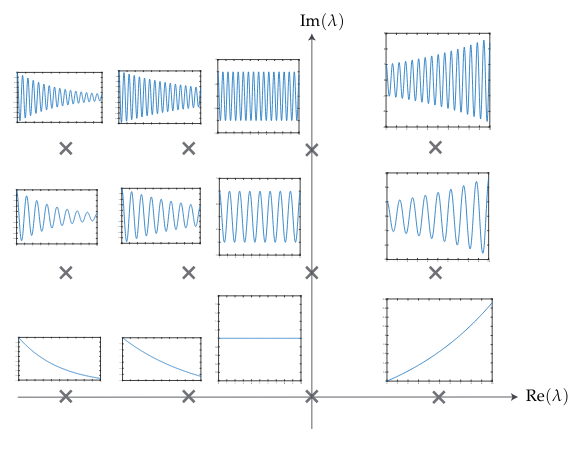
\includegraphics[width=\textheight]{continuous.png}
\end{frame}

\begin{frame}
    \frametitle{Stability}
    \framesubtitle{Discrete}
    
    \centering
    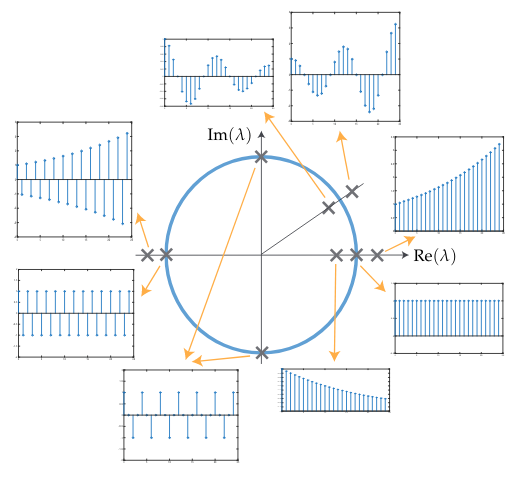
\includegraphics[width=\textheight]{discrete.png}
\end{frame}

\begin{frame}
    \frametitle{Controllability}

    \begin{align}
        \bm{x}[t + 1] &= \bm{Ax}[t] + \bm{Bu}[t] \\
        \bm{x}[1] &= \bm{Ax}[0] + \bm{Bu}[0] \\
        \bm{x}[2] &= \bm{A}^2 \bm{x}[0] + \bm{ABu}[0] + \bm{Bu}[1] \\
        \bm{x}[t] &= \bm{A}^t \bm{x}[0] + \sum_{i = 0}^{t - 1} \bm{A}^{t - i} \bm{Bu}[i] \\
        \bm{x}[t] - \bm{A}^t \bm{x}[0] &=
        \begin{bmatrix}
            \bm{B} & \bm{AB} & \cdots & \bm{A}^{t - 1} \bm{B}
        \end{bmatrix}
        \begin{bmatrix}
            \bm{u}[t - 1] \\
            \bm{u}[t - 2] \\ 
            \vdots \\
            \bm{u}[0]
        \end{bmatrix} \\
        \Rightarrow \operatorname{span}\left\{
        \begin{bmatrix}
            \bm{B} & \bm{AB} & \cdots & \bm{A}^{t - 1} \bm{B}
        \end{bmatrix}\right\} &= \R^n
    \end{align}
\end{frame}

\end{document}
